\documentclass{article}[12]

\usepackage{amsmath, amsthm, amssymb}
\usepackage{tikz}

\begin{document}

I'm Chris Grossack, and I study the geometric structure of certain groups of functions.
By this, I mean I have a bunch of functions that I carry around with me 
(who doesn't?) and I want to position my functions around me in a way that
makes sense (So randomly putting functions all over the place is not helpful,
I want to be meaningful with where I put things). I then want to use the
geometric structure of where the functions are positioned in order to better
understand the functions themselves.

If you'll indulge me, as a mathematician I feel obligated to say big words,
so I'll need to give some definitions. However, as a mathematician, I almost
never get to have as much fun with how I present definitions as I like, 
because it's not ``serious'' enough. I will try here to simultaneously
have fun, while still explaining what is happening.

\textbf{Definition:}
A \emph{binary string} is a (possibly infinte) sequence of $0$s and $1$s.
01101110011001010111001001100100, for instance, is a binary string.

\textbf{Definition:}
If I have a bunch of functions, this collection of functions is called a 
\emph{Group} of functions if it satisfies the following bonus properties:

\begin{enumerate}
  \item There is a fancy function called $I$ (for identity) so that \\
    for every $x$, $I(x) = x$.\\
    $I$ is the ``do nothing'' function,
    and it is in our collection.

  \item For any two functions in our bag, $f$ and $g$ there is another 
    function called $f + g$ which is also in our bag. Here,
    $(f + g)(x) = f(g(x))$. We also ask that addition not behave stupidly. \\
    Namely $(f + g) + h = f + (g + h)$, and $f + g = g + f$.
    
  \item For every function $f$ which is in our bag, there is another
    function in our bag (which I will suggestively call $-f$) 
    such that \\
    for every x, $f + (-f) = (-f) + f = I$ (that is, $-f$ undoes $f$).
\end{enumerate}

Now, to preemtively stop certain kinds of mathematicians from trying to
revoke my Math Card$^{\text{TM}}$, I am aware this makes us an \emph{Abelian}
Group, and is slightly less general than a regular group. To those who care, 
I kindly ask you to get over it.

There are lot of ways to define functions which are slightly more involved
than the standard definitions. For instance, here are the objects which
create the functions I study:

\textbf{Definition:}
A \emph{Finite State Automaton} is a machine like the one shown below:

\begin{center}
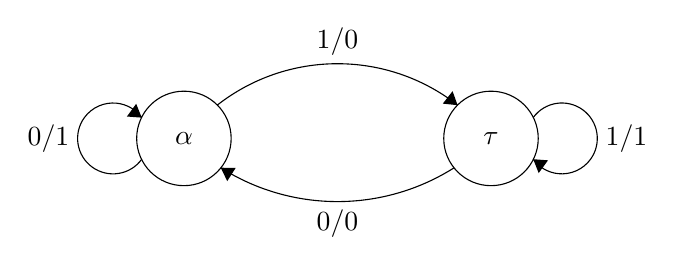
\begin{tikzpicture}[scale=0.2]
\tikzstyle{every node}+=[inner sep=0pt]
\draw [black] (15.8,-29.2) circle (3);
\draw (15.8,-29.2) node {$\alpha$};
\draw [black] (35.3,-29.2) circle (3);
\draw (35.3,-29.2) node {$\tau$};
\draw [black] (13.12,-30.523) arc (-36:-324:2.25);
\draw (8.55,-29.2) node [left] {$0/1$};
\fill [black] (13.12,-27.88) -- (12.77,-27) -- (12.18,-27.81);
\draw [black] (17.918,-27.085) arc (128.02449:51.97551:12.39);
\fill [black] (33.18,-27.09) -- (32.86,-26.2) -- (32.24,-26.99);
\draw (25.55,-23.96) node [above] {$1/0$};
\draw [black] (37.98,-27.877) arc (144:-144:2.25);
\draw (42.55,-29.2) node [right] {$1/1$};
\fill [black] (37.98,-30.52) -- (38.33,-31.4) -- (38.92,-30.59);
\draw [black] (32.957,-31.065) arc (-57.68311:-122.31689:13.856);
\fill [black] (18.14,-31.06) -- (18.55,-31.91) -- (19.09,-31.07);
\draw (25.55,-33.71) node [below] {$0/0$};
\end{tikzpicture}
\end{center}

These machines define functions which take in binary strings, and spit out
binary strings. The above machine, for instance, defines two functions,
$\alpha$ and $\tau$.

\end{document}
